\chapter{Implementace komponenty}
Navržená komponenta výukového serveru pro oblast TI byla realizována jako dynamická webová aplikace, která klade důraz na přehlednost, modularitu a interaktivní práci uživatele. Implementace vychází z rozdělení aplikace na samostatné logické celky, které zajišťují jak aplikační logiku, práci s~UI, tak i chování jednotlivých algoritmů. Důležitým aspektem tohoto řešení je propojení vizualizace s reálným průběhem výpočtu, kdy jsou jednotlivé kroky algoritmů přímo zobrazovány a aktualizovány prostřednictvím manipulace s DOM. Celá aplikace byla navržena tak, aby byla snadno rozšiřitelná, přehledná z pohledu implementace a zároveň vhodná pro praktické využití ve výuce.


\section{Použité technologie a vývojové prostředí}
Implementace komponenty byla realizována jako dynamická webová aplikace s využitím technologií HTML, CSS a JS. Jazyk HTML slouží pro definici struktury celé stránky, CSS pro její vizuální styl a responzivní zobrazení a JS pro zajištění aplikační logiky. Dynamická práce s obsahem stránky je realizována prostřednictvím manipulace s DOM, což umožňuje aktualizaci jednotlivých částí UI bez nutnosti opětovného načítání celé stránky. Pro vizuální animační efekty v pozadí stránky bylo využito také Canvas API \cite{canvas_api}.

V implementaci byly také využity vybrané knihovny, které usnadnily práci s UI. Pro stylování a~rozložení stránky byla použita knihovna Bootstrap \cite{bootstrap}, pro práci s ikonami knihovna Font Awesome \cite{font_awesome} a pro vybrané části klientské logiky knihovna jQuery \cite{jquery}. Aplikace nevyužívá žádné externí API, veškerá logika je realizována na straně klienta.

Celá praktická část byla vyvíjena v prostředí Visual Studio Code, které sloužilo pro implementaci aplikace. Teoretická část práce byla zpracována pomocí systému \LaTeX{} v prostředí Overleaf.


\section{Struktura a realizace aplikace}
Aplikace je rozdělena do více zdrojových souborů podle jejich účelu. Toto rozdělení zlepšuje přehlednost implementace, odděluje společné části od specializovaných modulů a usnadňuje další úpravy i~rozšiřování celé aplikace.

\subsection{Organizace zdrojových souborů}
Zdrojové soubory jsou rozděleny na hlavní stránku, sdílené prostředky, aplikační logiku, zpracování vstupních režimů a moduly jednotlivých algoritmů. Díky tomu lze snadno rozlišit, která část zajišťuje konkrétní chování aplikace.

\begin{itemize}
    \item \texttt{index.html} -- hlavní struktura stránky
    \item \texttt{styles.css} -- vzhled a responzivita
    \item \texttt{animation.js} -- animované pozadí stránky
    \item \texttt{translations.js} -- jazykové překlady aplikace
    \item \texttt{state\_app.js} -- globální stav aplikace
    \item \texttt{language\_app.js} -- přepínání jazyků
    \item \texttt{modals\_app.js} -- obsluha modálních oken
    \item \texttt{navigation\_app.js} -- navigace mezi částmi
    \item \texttt{theme\_app.js} -- vzhledové nastavení
    \item \texttt{init\_app.js} -- inicializace aplikace
    \item \texttt{helpers\_typesParams.js} -- pomocné funkce vstupů
    \item \texttt{manual\_typesParams.js} -- ruční zadávání vstupu
    \item \texttt{random\_typesParams.js} -- náhodné generování vstupu
    \item \texttt{specialCases\_typesParams.js} -- ukázkové speciální případy
    \item \texttt{syntax\_typesParams.js} -- vstup pomocí příkazů
    \item \texttt{state\_multipop.js} -- globální stav algoritmu Multipop na zásobníku
    \item \texttt{ui\_multipop.js} -- rozhraní algoritmu Multipop na zásobníku
    \item \texttt{manual\_multipop.js} -- ruční režim algoritmu Multipop na zásobníku
    \item \texttt{actions\_multipop.js} -- operace algoritmu Multipop na zásobníku
    \item \texttt{syntax\_multipop.js} -- syntaxe algoritmu Multipop na zásobníku
    \item \texttt{random\_multipop.js} -- náhodný režim algoritmu Multipop na zásobníku
    \item \texttt{specialCases\_multipop.js} -- speciální případy algoritmu Multipop na zásobníku
    \item \texttt{state\_queue2Stacks.js} -- globální stav algoritmu Fronta pomocí dvou zásobníků
    \item \texttt{ui\_queue2Stacks.js} -- rozhraní algoritmu Fronta pomocí dvou zásobníků
    \item \texttt{manual\_queue2Stacks.js} -- ruční režim algoritmu Fronta pomocí dvou zásobníků
    \item \texttt{actions\_queue2Stacks.js} -- operace algoritmu Fronta pomocí dvou zásobníků
    \item \texttt{syntax\_queue2Stacks.js} -- syntaxe algoritmu Fronta pomocí dvou zásobníků
    \item \texttt{random\_queue2Stacks.js} -- náhodný režim algoritmu Fronta pomocí dvou zásobníků
    \item \texttt{specialCases\_queue2Stacks.js} -- speciální případy algoritmu Fronta pomocí dvou zásobníků
    \item \texttt{state\_splayTree.js} -- globální stav algoritmu Splay strom
    \item \texttt{ui\_splayTree.js} -- rozhraní algoritmu Splay strom
    \item \texttt{manual\_splayTree.js} -- ruční režim algoritmu Splay strom
    \item \texttt{actions\_splayTree.js} -- operace algoritmu Splay strom
    \item \texttt{syntax\_splayTree.js} -- syntaxe algoritmu Splay strom
    \item \texttt{random\_splayTree.js} -- náhodný režim algoritmu Splay strom
    \item \texttt{specialCases\_splayTree.js} -- speciální případy algoritmu Splay strom
\end{itemize}

\subsection{Hlavní části aplikační logiky}
Velmi důležitou součástí implementace je hlavní aplikační logika, která zajišťuje propojení jednotlivých částí celé aplikace. Tato vrstva se stará zejména o správu globálního stavu, změny zobrazeného obsahu, aktualizaci rozhraní a návaznost mezi jednotlivými moduly. Právě díky této části aplikace spolu mohou správně spolupracovat sdílené prvky, jednotlivé algoritmy i různé režimy spuštění.

Jako ukázka hlavní aplikační logiky byla vybrána funkce \texttt{changeLanguage()}. Tato funkce se nachází v souboru \texttt{language\_app.js}. Její výběr je vhodný proto, že dobře ukazuje centrální řízení aplikace, protože při změně jazyka neaktualizuje pouze texty v rozhraní, ale také pracuje s uloženým nastavením, mění jazyk dokumentu, obnovuje aktuální zobrazení aplikace a zajišťuje správnou aktualizaci otevřených modálních oken i dalších aktivních prvků.

\begin{lstlisting}[language=Java, caption={Ukázka hlavní aplikační logiky ve funkci changeLanguage()}, label={lst:change_language}]
function changeLanguage(language){
  closeNavbarMenu();
  localStorage.setItem('language', language);
  document.documentElement.lang = language === 'cz' ? 'cs' : 'en';

  const Lall = trAll(language);

  langAppApplyCommonStaticTexts(Lall);
  langAppApplyAccessibilityTexts(Lall);
  langAppApplyAlgorithmSelectionTexts(Lall);
  langAppApplyPageTexts(language, Lall);
  langAppApplyParameterButtonTexts(Lall);
  langAppApplyManualModalTexts(Lall, language);
  langAppApplyRandomModalTexts(language, Lall);
  langAppApplySyntaxModalTexts(Lall);
  langAppApplySpecialCasesModalTexts(Lall);

  refreshCurrentViewAfterLanguageChange();
  langAppRefreshRandomOperationPreviews();

  if(typeof refreshOpenTransientModalsForLanguage === 'function')
    refreshOpenTransientModalsForLanguage();
  if(typeof refreshOpenSpecialCasesModalForLanguage === 'function')
    refreshOpenSpecialCasesModalForLanguage();
  if(typeof refreshOpenHistoryModalForLanguage === 'function')
    refreshOpenHistoryModalForLanguage();
  if(typeof updateThemeToggleUI === 'function')
    updateThemeToggleUI();
}
\end{lstlisting}
\addcontentsline{lof}{figure}{\protect\numberline{\thelstlisting}Ukázka hlavní aplikační logiky ve funkci changeLanguage()}

Na uvedené ukázce \ref{lst:change_language} je vidět, že hlavní aplikační logika není omezena jen na jednu dílčí činnost, ale propojuje více částí systému současně. Funkce nejprve uloží zvolený jazyk, následně upraví jazyk dokumentu a poté aktualizuje textové prvky celého rozhraní. Současně zajistí obnovení právě zobrazené části aplikace a případně i aktualizaci otevřených modálních oken nebo dalších aktivních prvků. Tento způsob řešení podporuje centralizaci důležité logiky na jednom místě a~zároveň usnadňuje správu i další rozšiřování aplikace.

\subsection{Implementace vybraných algoritmů}
V praktické části byly implementovány tři algoritmy: \textit{Multipop on Stack}, \textit{Queue using Two Stacks} a \textit{Splay Tree}. Každý z nich reprezentuje jiný typ chování vhodný pro amortizovanou analýzu. První algoritmus pracuje se zásobníkem založeným na principu LIFO, druhý simuluje frontu s principem FIFO pomocí dvou zásobníků a třetí algoritmus vychází z vlastností binárního vyhledávacího stromu BST, který se při operacích dynamicky přizpůsobuje. Z důvodu přehlednosti nejsou v této podkapitole uvedeny celé implementace algoritmů, ale pouze vybrané a zkrácené ukázky kódu, na kterých je dobře vidět hlavní princip jejich realizace.

Jako první ukázka byla vybrána část implementace algoritmu \textit{Multipop on Stack}, konkrétně operace \texttt{multipopFromStackManual(count)} ze souboru \texttt{manual\_multipop.js}. Tato ukázka byla zvolena proto, že přímo vystihuje hlavní princip algoritmu, tedy odebrání více prvků ze zásobníku najednou, přičemž skutečný počet odebraných prvků závisí na aktuálním stavu zásobníku.

\begin{lstlisting}[language=Java, caption={Zkrácená ukázka implementace operace multipop}, label={lst:multipop_impl}]
function multipopFromStackManual(count){
  if(mpBusy)
    return null;

  const beforeState = mpCreateStateSnapshot();
  const actualCount = Math.min(count, beforeState.size);

  if(actualCount === 0)
    return [];

  const removedValues = beforeState.snapshot.slice(-actualCount);
  const afterSnapshot = beforeState.snapshot.slice(0, beforeState.size - actualCount);

  mpApplyManualStateAndRefresh(
    afterSnapshot,
    beforeState.stepCount + actualCount,
    afterSnapshot.length
  );

  return removedValues;
}
\end{lstlisting}
\addcontentsline{lof}{figure}{\protect\numberline{\thelstlisting}Zkrácená ukázka implementace operace multipop}

Na ukázce \ref{lst:multipop_impl} je vidět, že implementace nejprve zjistí aktuální stav zásobníku a následně určí skutečný počet prvků, které lze odebrat. Ten je omezen minimem mezi požadovaným počtem a aktuální velikostí zásobníku. Právě tato vlastnost dobře vystihuje rozdíl mezi požadovanou a skutečně provedenou prací, což je pro tento algoritmus z hlediska amortizované analýzy podstatné.

Jako druhá ukázka byla vybrána část implementace algoritmu \textit{Queue using Two Stacks}. Konkrétně jde o funkci \texttt{qTransferAllFromInToOut(done)} ze souboru \texttt{manual\_queue2Stacks.js}. Tato ukázka byla zvolena proto, že zachycuje klíčový mechanismus celé struktury, tedy přesun prvků ze vstupního zásobníku do výstupního zásobníku.

\begin{lstlisting}[language=Java, caption={Zkrácená ukázka přesunu prvků při implementaci fronty pomocí dvou zásobníků}, label={lst:queue_transfer_impl}]
function qTransferAllFromInToOut(done){
  if(qIn.length === 0){
    qPotential = qIn.length;
    updateQueueCounters();
    
    if(done)
      done();
    return;
  }

  const value = qIn[qIn.length - 1];
  qAnimateRemoveTopItem('qInView', () => {
    qIn.pop();
    qStepCount += 1;

    qOut.push(value);
    qStepCount += 1;
    qPotential = qIn.length;
    
    renderQueueStacks();
    qAnimateAddTopItem('qOutView');
    updateQueueCounters();

    qRunTimer = setTimeout(() => {
      qTransferAllFromInToOut(done);
    }, qSkipAnimations ? 0 : 250);
  });
}
\end{lstlisting}
\addcontentsline{lof}{figure}{\protect\numberline{\thelstlisting}Zkrácená ukázka přesunu prvků při implementaci fronty pomocí dvou zásobníků}

Ukázka \ref{lst:queue_transfer_impl} vystihuje princip, na kterém je založena realizace fronty pomocí dvou zásobníků. Pokud je výstupní zásobník prázdný, prvky se postupně přesouvají ze vstupního zásobníku, čímž dojde k obrácení jejich pořadí. Právě tímto způsobem je možné zajistit chování odpovídající principu FIFO, přestože vnitřně aplikace pracuje se dvěma zásobníky.

Jako třetí ukázka byla vybrána část implementace algoritmu \textit{Splay Tree}, konkrétně funkce \texttt{sRotateLeft(node)} ze souboru \texttt{manual\_splayTree.js}. Tato ukázka byla zvolena proto, že rotace představují základní mechanismus, pomocí kterého se splay strom při operacích strukturálně upravuje.

\begin{lstlisting}[language=Java, caption={Zkrácená ukázka levé rotace ve splay stromu}, label={lst:splay_rotate_left}]
function sRotateLeft(node){
  const rightChild = node.right;
  if(!rightChild)
    return;

  sStepCount += 1;

  node.right = rightChild.left;
  if(rightChild.left)
    rightChild.left.parent = node;

  rightChild.parent = node.parent;

  if(!node.parent)
    sRoot = rightChild;
  else if(node === node.parent.left)
    node.parent.left = rightChild;
  else
    node.parent.right = rightChild;

  rightChild.left = node;
  node.parent = rightChild;
}
\end{lstlisting}
\addcontentsline{lof}{figure}{\protect\numberline{\thelstlisting}Zkrácená ukázka levé rotace ve splay stromu}

Na ukázce \ref{lst:splay_rotate_left} je vidět, jak se při levé rotaci mění vazby mezi vrcholy stromu. Přestože jde jen o zkrácenou část implementace, dobře ukazuje, že splay strom není založen pouze na běžném vyhledávání ve struktuře BST, ale také na dynamické změně jejího tvaru pomocí rotací. Právě tyto strukturální úpravy jsou pro chování splay stromu a jeho amortizovanou analýzu zásadní.

\subsection{Zpracování vstupů a režimů spuštění}
Důležitou součástí implementace je také zpracování vstupů a jednotlivých režimů spuštění aplikace. Uživatel může pracovat s několika způsoby zadání, konkrétně ručním vstupem, náhodně generovaným vstupem, vstupem pomocí syntaxe a připravenými speciálními případy. Pro přehlednost a znovupoužitelnost byla tato část řešena pomocí společné vrstvy \texttt{typesParams}, která sjednocuje obsluhu jednotlivých typů vstupů pro všechny implementované algoritmy.

Jako ukázka zpracování vstupů a režimů spuštění byla vybrána zkrácená část konfigurace. Konkrétně jde o \texttt{ALG\_REGISTRY}. Ukázka přehledně zachycuje, jak jsou pro jednotlivé algoritmy definovány dostupné režimy spuštění. Současně je na ní vidět, jak je nad těmito režimy vystavěna společná obslužná vrstva. Z ukázky je také patrné, že aplikace neřeší každý algoritmus zcela samostatně, ale používá jednotný princip pro ruční vstup, náhodné generování, speciální případy i syntax režim.

\begin{lstlisting}[language=Java, basicstyle=\ttfamily\scriptsize, breaklines=true, columns=fullflexible, caption={Zkrácená ukázka konfigurace vstupních režimů}, label={lst:types_params_registry}]
const ALG_REGISTRY = Object.freeze({
  multipop: {
    contexts: {manual: 'multipopManual', random: 'multipopRandom', specialCases: 'multipopSpecialCases', syntax: 'multipopSyntax'},
    manual: {type: 'stackModal', start: typesParamsStartMultipopWithValues},
    random: {type: 'randomModal', start: typesParamsStartMultipopRandomMode},
    specialCases: {getScenarios: typesParamsGetMultipopSpecialScenarios, start: typesParamsRunMultipopSpecialScenario},
    syntax: {resetBeforeOpen: typesParamsResetMultipopSyntaxState, start: typesParamsStartMultipopSyntax}
  },
  queue2Stacks: {
    contexts: {manual: 'queueManual', random: 'queueRandom', specialCases: 'queueSpecialCases', syntax: 'queueSyntax'},
    manual: {type: 'stackModal', start: typesParamsStartQueueWithValues},
    random: {type: 'randomModal', start: typesParamsStartQueueRandomMode},
    specialCases: {getScenarios: typesParamsGetQueueSpecialScenarios, start: typesParamsRunQueueSpecialScenario},
    syntax: {resetBeforeOpen: typesParamsResetQueueSyntaxState, start: typesParamsStartQueueSyntax}
  },
  splayTree: {
    contexts: {manual: 'splayManual', random: 'splayRandom', specialCases: 'splaySpecialCases', syntax: 'splaySyntax'},
    manual: {type: 'actionInput', titleKey: 'splayInitTitle', labelKey: 'splayInitLabel', infoKey: 'splayInitInfo', invalidKey: 'splayInitInvalid', start: typesParamsStartSplayManualWithValues},
    random: {type: 'randomModal', start: typesParamsStartSplayRandomMode},
    specialCases: {getScenarios: typesParamsGetSplaySpecialScenarios, start: typesParamsRunSplaySpecialScenario},
    syntax: {start: typesParamsStartSplaySyntax}
  }
});
\end{lstlisting}
\addcontentsline{lof}{figure}{\protect\numberline{\thelstlisting}Zkrácená ukázka konfigurace vstupních režimů}

Na ukázce \ref{lst:types_params_registry} je vidět, že vrstva \texttt{typesParams} sjednocuje obsluhu všech hlavních režimů spuštění aplikace. Pro každý algoritmus jsou zde definovány kontexty jednotlivých režimů, tedy manuální vstup, náhodný vstup, speciální případy a syntax režim. Současně je zde určeno, jaký typ vstupního rozhraní se má použít a která funkce zajistí samotné spuštění zvoleného režimu. Toto řešení přispívá k větší modularitě aplikace, protože společná logika zpracování vstupů není duplikována v každém algoritmu zvlášť. Vrstva \texttt{typesParams} tak tvoří rozhraní mezi uživatelským zadáním a konkrétní implementací jednotlivých algoritmů.


\section{Uživatelské rozhraní a responzivita}
UI je důležitou částí celé aplikace, protože zprostředkovává práci s algoritmy, vstupy i jednotlivými režimy spuštění. Současně bylo nutné navrhnout jej tak, aby zůstalo přehledné při dynamických změnách obsahu a bylo použitelné i na různých typech zařízení.

\subsection{Struktura uživatelského rozhraní a práce s dynamickým obsahem}
Součástí implementace je návrh struktury UI a způsob, jakým je do stránky vkládán a měněn dynamický obsah. Aplikace není vytvořena jako sada více samostatných statických stránek, ale jako jedna hlavní dynamická stránka, ve které se podle zvoleného algoritmu a režimu spuštění mění zobrazovaný obsah přímo v rámci DOM.

Jako ukázka byla vybrána zkrácená část HTML struktury z těla dokumentu. Tato ukázka pochází ze souboru \texttt{index.html}. Přehledně zachycuje hlavní navigaci, výběr algoritmů, prostor pro dynamicky vkládaný obsah, modální okna i další prvky rozhraní.

\begin{lstlisting}[language=XML, basicstyle=\ttfamily\scriptsize, breaklines=true, columns=fullflexible]
<body>
  <canvas id="bgCanvas" aria-hidden="true"></canvas>
  
  <!-- Hlavni navigace -->
  <nav class="navbar ..." >
    ...
    <button id="aboutAppBtn" ...>...</button>
    <div id="backArrow">
      <button id="backBtn" ...>...</button>
    </div>
  </nav>
  
  <!-- Vyber algoritmu -->
  <div class="alg-panel" id="algorithmLinks">
    ...
    <button id="algorithm1" onclick="changeContent('multipop')">...</button>
    <button id="algorithm2" onclick="changeContent('queue2Stacks')">...</button>
    <button id="algorithm3" onclick="changeContent('splayTree')">...</button>
  </div>

  <!-- Dynamicky obsah -->
  <div id="dynamicContent" class="text-center mt-5"></div>
\end{lstlisting}
\newpage
\noindent\textit{Pokračování ukázky kódu.}
\begin{lstlisting}[language=XML, basicstyle=\ttfamily\scriptsize, breaklines=true, columns=fullflexible, caption={Zkrácená ukázka struktury uživatelského rozhraní v souboru index.html}, label={lst:index_body_ui}]
  <!-- Priklad modalniho okna -->
  <div class="modal fade" id="aboutModal" ...>
    <div class="modal-dialog ...">
      <div class="modal-content">
        <div class="modal-header">
          <h5 id="aboutModalLabel"></h5>
        </div>
        <div class="modal-body" id="aboutModalBody"></div>
        <div class="modal-footer">
          <button id="closeBtn" ...></button>
        </div>
      </div>
    </div>
  </div>

  <!-- Dalsi modalni okna -->
  ...
  <footer>
    ...
    <button id="themeToggle" class="theme-toggle"></button>
    <span id="footerText"></span>
  </footer>

  <!-- Nacteni JS souboru -->
  <script src="..."></script>
  ...
</body>
\end{lstlisting}
\phantomsection
\addcontentsline{lof}{figure}{\protect\numberline{\thelstlisting}Zkrácená ukázka struktury uživatelského rozhraní v souboru index.html}

Na ukázce \ref{lst:index_body_ui} je vidět, že uživatelské rozhraní je postaveno na jedné společné HTML kostře. Ta obsahuje hlavní navigaci, úvodní panel pro výběr algoritmů, centrální prvek \texttt{dynamicContent} určený pro dynamicky vkládaný obsah, sadu modálních oken a také patičku s dalšími ovládacími prvky. Právě element \texttt{dynamicContent} slouží jako hlavní prostor, do kterého aplikace podle aktuální situace vkládá nové části rozhraní. Současně je z ukázky patrné, že důležitou roli hrají i modální okna, která slouží pro zadávání vstupních parametrů, zobrazení doplňujících informací nebo práci s historií kroků. Významná je také návaznost na načítané JS soubory.
\newpage

\subsection{Responzivní zobrazení na různých zařízeních}
V průběhu návrhu celé aplikace byl brán ohled také na responzivní zobrazení na mobilních zařízeních, i když tato část nebyla přímo požadována v zadání. Cílem bylo, aby aplikace zůstala použitelná a přehledná nejen na běžném monitoru, ale i na menších obrazovkách.

Na obrázku \ref{fig:responsive_ui_compare} je zachyceno porovnání hlavní stránky na desktopovém a mobilním zařízení. Ze srovnání je patrné, že aplikace si zachovává stejné základní prvky rozhraní, ale jejich rozmístění a velikost se přizpůsobují dostupnému prostoru obrazovky.

\begin{figure}[H]
    \centering
    \subfloat[Hlavní stránka aplikace na desktopovém zařízení]{%
        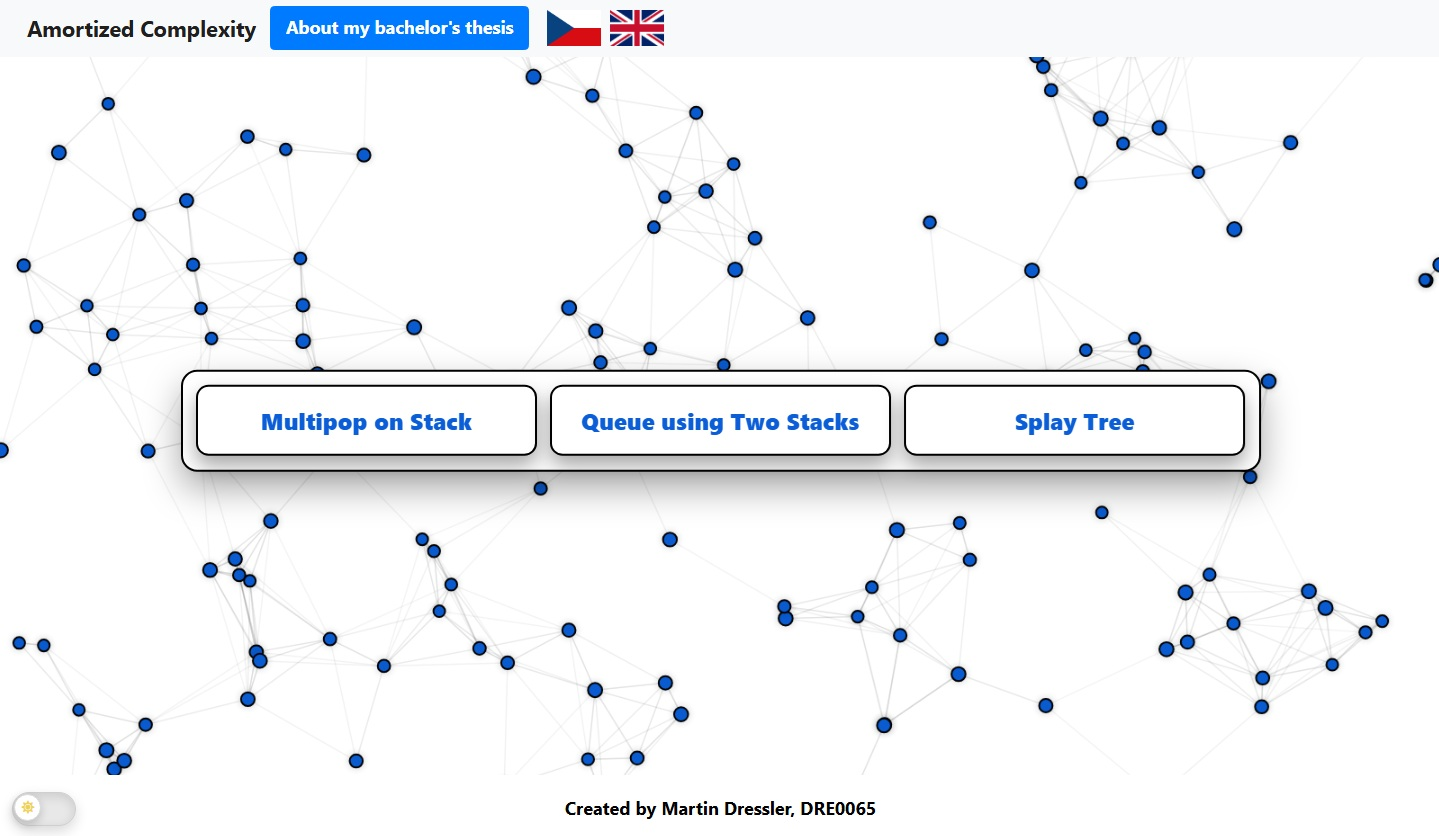
\includegraphics[width=0.7\textwidth]{Figures/main_page_algorithm_selection.jpg}}
    \hfill
    \subfloat[Hlavní stránka aplikace na mobilním zařízení]{%
        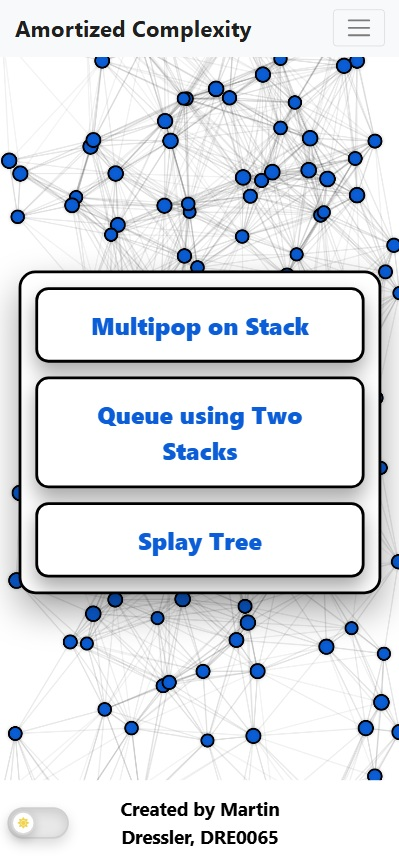
\includegraphics[width=0.3\textwidth]{Figures/mobile_main_page.jpg}}
    \caption{Porovnání zobrazení hlavní stránky na různých typech zařízení}
    \label{fig:responsive_ui_compare}
\end{figure}
\newpage

Responzivní chování bylo řešeno v souboru \texttt{styles.css} pomocí pravidel \texttt{@media}.

\begin{lstlisting}[basicstyle=\ttfamily\footnotesize, breaklines=true, columns=fullflexible, caption={Zkrácená ukázka responzivních pravidel pro mobilní zařízení}, label={lst:responsive_media_query}]
@media(max-width: 767.98px){
  ...
}
\end{lstlisting}
\addcontentsline{lof}{figure}{\protect\numberline{\thelstlisting}Zkrácená ukázka responzivních pravidel pro mobilní zařízení}

Na ukázce \ref{lst:responsive_media_query} je vidět, že pro menší obrazovky byla použita samostatná část stylů, která upravuje zobrazení aplikace pro mobilní zařízení. Díky tomu bylo možné zachovat přehlednost rozhraní i při výrazně menším dostupném prostoru.


\section{Nasazení a zpřístupnění aplikace}
Po dokončení implementace byla aplikace nasazena a zpřístupněna prostřednictvím školního serveru Homel, který se jevil jako nejvhodnější řešení pro hosting. Díky tomu je možné práci snadno veřejně zpřístupnit v rámci univerzitního prostředí a současně je zajištěn jednoduchý způsob, jak aplikaci prezentovat, testovat a dále využívat.

Pro spuštění aplikace není potřeba instalovat žádné další balíčky ani knihovny. Pro správnou funkci je nutné zachovat původní strukturu odevzdané praktické části, zejména adresáře \texttt{css}, \texttt{html}, \texttt{images} a \texttt{js}, protože aplikace využívá relativní cesty mezi soubory. Pro lokální spuštění stačí otevřít soubor \texttt{index.html} z adresáře \texttt{html} ve webovém prohlížeči. Knihovny Bootstrap, Font Awesome a~jQuery jsou připojeny prostřednictvím CDN, takže při spuštění je potřeba internetové připojení, aby se tyto prostředky mohly načíst. Není třeba upravovat žádné konfigurační soubory ani provádět sestavení aplikace, protože veškerá logika je realizována na straně klienta.

Výsledná aplikace je v době odevzdání bakalářské práce dostupná prostřednictvím protokolu HTTP na adrese URL \url{https://homel.vsb.cz/~dre0065/DRE0065_BP/html/}.